\cotefile{162-5}
\scanpage{3}
\mspage{1}
\margin{\handwritten{notes du \uline{10.9.68}}}

Tapis de Quillen.

I \quad \uline{Relations entre catégories et ensembles semi-simpliciaux}.

A toute catégorie $C$, on associe un ensemble semi-simpli\unsure{\deleted{v}c|\deleted{c}v}ial $S(C)$,
trouvant \unsure{\deleted{n}a|\deleted{a}n}\unsure{\deleted{n}i|\deleted{i}n}nsi un foncteur pleinement fidèle \deleted{de Cat}
\[
S;\ (\mathrm{Cat}) \longrightarrow (\mathrm{Ssimpl}) \quad .
\]
\deleted{Si $C$ est associé à} Les systêmes locaux d'ensemble sur $SC$ correspondent
aux f\unsure{\deleted{a}o|a}ncteurs sur $C$ qui transforment toute flêche en isomorphisme (i.e.
qu\unsure{\deleted{b}i|\deleted{t}i|\deleted{i}b} se factorisent par le groupoïde associé à $C$). Les $H^i$ sur $SC$ d'un tel
systême local ($H^o$ pour ens, $H^1$ pour groupes, $H^i$ quelconques pour groupes
abéliens) s'interprètent en termes des foncteurs $\varprojlim^{(i)}$ déri\unsure{\deleted{g}v|\deleted{v}g}és de $\varprojlim$,
ou si on préfère, des $H^i($ du \uline{topos} $\unsure{C^{\wedge}|C}$. On voit ainsi à quelle condition
un foncteur $C\longrightarrow C'$ induit un\deleted{e} homotopisme $SC\longrightarrow SC'$ : en vertu du
critère cohomologique de Artin-Mazur, il f et s que pour tout systême
de coéfficients $F'$sur $C'$, l'homomorphisme naturel $\varprojlim_{C'}^{(i)}F'\longrightarrow\varprojlim_C^{(i)}F$
soit un isomorphisme (pour les $i$ pour lesquels cela a un sens). \deleted{\unsure{Premiers|Exemples}}

A $C$ on peut asso\unsure{\deleted{v}c|\deleted{c}v}\unsure{\deleted{e}i|\deleted{i}e}r le topos $\widetilde C$, qui varie de façon \uline{covariante} avec $C$
(NB le foncteur $C\longmapsto\widetilde C$ n'a plus rien de pleinement fidèle, semble-til ??)
Les systêmes de coéfficients \begin{tabular}[b]{@{}l@{}}\inserted{ensemblistes}\\[-.65ex]\begin{tikzpicture}[x=1em,y=1em,baseline=0pt]\draw[line width=.5pt] (7.8,.8) .. controls (8.1,.05) and (6.6,-.2) .. (3.4,-.2) .. controls (3,-.12) and (2.9,-.2) .. (2.9,-.9);\end{tikzpicture}\end{tabular} sur $C$ ( $\overset{\inserted{\mathrm{déf}}}{=}$ les foncteurs \begin{tabular}[b]{@{}l@{}}\inserted{$C^o\longrightarrow\mathrm{Ens}$}\\[-.6ex]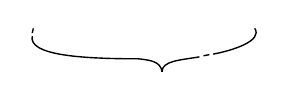
\begin{tikzpicture}[x=1em,y=1em,baseline=0pt]\draw[line width=.5pt] (0,.65) -- (-.04,.48);\draw[line width=.5pt] (-.04,.37) .. controls (-.18,-.3) and (1.6,-.45) .. (3.8,-.45) .. controls (4.25,-.5) and (4.6,-.55) .. (4.65,-.92);\draw[line width=.5pt] (8,.65) .. controls (8.3,.2) and (7.2,-.15) .. (6.5,-.28);\draw[line width=.5pt] (6.36,-.3) -- (6.15,-.34);\draw[line width=.5pt] (6,-.38) .. controls (5.3,-.5) and (4.65,-.52) .. (4.65,-.92);\end{tikzpicture}\end{tabular} transformant isomo\unsure{r}phismes en isomorphismes) correspondent aux faisceaux localement constant
i.e. les objets localement constants de $\widetilde C$, définis intrinsèquement en te\unsure{r}
de $\widetilde C$. Ainsi, le fait pour un foncteur $F:C\longrightarrow C'$ d'induire un\deleted{e \unsure{équivalence}}
homotopisme $S(C)\longrightarrow S(C')$ ne dépend que du morphisme de topos $\widetilde F:\widetilde C\longrightarrow\widetilde C'$
induit, et signifie que pour tout faisceau localement constant $F'$ sur $C'$
\unsure{c.|e.} sur $\widetilde C'$, les applic\unsure{a}tions induites $H^i(\widetilde C',F')\longrightarrow H^i(\widetilde C,\widetilde F^*.(F'))$
sont des isomorphismes (pour les $i$ pour lesquels cela a un\deleted{e\unsure{n|m}} sens).

\margin{2}
